% Introduction

\vspace{21.5pt}
\chapter{Introduction}\label{sec:sec_introduction}

Embedded systems are specialized computer systems designed to perform specific tasks or functions
within a larger system~\cite{muench2018you}. They are essential for many devices
and applications, making things work smoothly and efficiently in our everyday
lives. These systems tightly integrate hardware and software components to optimize performance,
power consumption, and system size~\cite{eisele2022embedded}. The importance of embedded systems
lies in their ubiquity and versatility. They are found in numerous devices and industries,
including consumer electronics~\cite{andrae2010life}, telecommunications~\cite{paulin1995dsp},
automotive~\cite{Automoti68:online}, aerospace~\cite{bieber2012security},
medical~\cite{jafari2007medical}, and industrial automation~\cite{thramboulidis2007soa}.
Examples of embedded systems include microcontrollers~\cite{gridling2007introduction} in
smart home appliances~\cite{kang2017enhanced}, digital signal processors in wireless
communication devices~\cite{kostic1997digital}, control systems in autonomous
vehicles~\cite{kostic1997digital}, and sensor networks for monitoring and
automation~\cite{marwedel2021embedded}. This is just to show some applications of
embedded systems as this list is far from exhaustive


As the world gets more connected and depends more on technology, embedded
systems are becoming even more important. They are essential for
enabling the \gls{iot}, robotics, medical instruments, and smart cities~\cite{camposano1996embedded:ARTICLE}.
As of February 2023, an estimated 21.5 billion interconnected devices
exist worldwide, according to Statista~\cite{IoTconne16:online}~\cite{HowManyI1:online}.
This number is expected to continue increasing as internet consumption rises, and
new devices and machinery are introduced to the market. By 2025, it's expected
that about 75.44 billion IoT (Internet of Things) devices will be set up all
over the world~\cite{HowManyI1:online}.

The number of embedded devices per person is significantly higher in developed
countries than in developing nations. For instance, in
the United States, there were about 13 \acrshort{iot} devices for each
person in 2020~\cite{Stateoft48:online}.
In comparison, the global average was around 3.5 \acrshort{iot} devices per person during
the same year~\cite{CiscoAnn1:online}. In developed countries, prevalent devices
typically include intelligent home appliances~\cite{wang2015anycontrol},
wearable technology~\cite{poongodi2020wearable}, and
interconnected vehicles~\cite{priyan2019survey}~\cite{Internet36:online}.
Conversely, in developing countries, there is a notable focus on deploying
devices that support key sectors such as
agriculture~\cite{baranwal2016development}, healthcare~\cite{pradhan2021iot},
and the monitoring of critical infrastructure~\cite{patil2012internet}.

The rapid growth of embedded systems calls for strong security, reliability, and
efficiency to keep the technology we use daily safe and working properly~\cite{muench2018you}.
Mirai malware attacks have demonstrated their potential for large-scale disruption, targeting devices like
routers, cameras, and DVRs to execute \gls{DDOS} attacks~\cite{KrebsOnS42:online}~\cite{antonakakis2017understanding}.
In 2016, a \acrshort{DDOS} attack on Dyn~\cite{LargeDDo94:online}, a DNS provider, significantly
hindered user access to prominent services such as Twitter, Amazon, Tumblr, Reddit, Spotify, and
Netflix~\cite{muench2018you}~\cite{lindqvist2017future}. \textit{Ripple20},
a group of 19 serious weaknesses found in the Treck TCP/IP library~\cite{TreckTCP63:online},
impacted IoT devices used in industrial control systems, healthcare devices,
and home appliances. The vulnerabilities known as URGENT/11~\cite{WhatisUR60:online}
and BadAlloc~\cite{IoTriddl27:online}, identified in the VxWorks
\gls{rtos}~\cite{VxWorksI53:online}, have impacted millions of embedded devices.
These devices range from medical equipment and industrial control systems to
routers~\cite{seri2019critical}. Stemming from flaws in memory allocation
functions, these vulnerabilities could enable remote code execution, thus
permitting attackers to gain control over the affected
devices~\cite{1NewMess42:online}.

In the digital age, data breaches have become a common problem, affecting
individuals, businesses, and governments~\cite{10oftheB31:online},
the following Table:~\ref{tab:data_breaches} points out some of the biggest data
breaches that have happened in the 21st century~\cite{The15big77:online}~\cite{10oftheB31:online}.
These events remind us how important strong cybersecurity is and that we always
need to be careful in protecting private information.

\begin{table}[ht]
      \centering
      \caption{Data Breaches in the 21st Century}
      \label{tab:data_breaches}
      \begin{tabularx}{\textwidth}{|l|X|}
      \hline
      \textbf{Company} & \textbf{Description} \\
      \hline
      Yahoo & In 2013 and 2014, Yahoo experienced two significant data breaches affecting approximately 3 billion user accounts. The breaches exposed users' personal information, including names, email addresses, and hashed passwords. \\
      \hline
      Equifax & In 2017, Equifax, a major credit reporting agency, suffered a data breach compromising the personal data of approximately 147 million Americans, exposing sensitive information such as Social Security numbers, birth dates, and addresses. \\
      \hline
      Marriott International & In 2018, Marriott disclosed a data breach affecting approximately 500 million customers. The breach involved unauthorized access to the Starwood guest reservation database, exposing personal details, passport numbers, and payment card information. \\
      \hline
      Capital One & In 2019, Capital One's systems were accessed by a hacker, resulting in the exposure of personal information of approximately 106 million individuals in the United States and Canada, including names, addresses, credit scores, and Social Security numbers. \\
      \hline
      Facebook/Cambridge Analytica & In 2018, Cambridge Analytica harvested personal data from millions of Facebook users without their consent, raising concerns about privacy and data protection on social media platforms. \\
      \hline
      Target & In 2013, Target experienced a breach affecting approximately 41 million customer payment card accounts. The attack exploited vulnerabilities in the company's payment system, resulting in the theft of credit and debit card information. \\
      \hline
      \end{tabularx}
\end{table}


Software testing~\cite{myers2011art} is a very important step in making embedded
systems, especially as the number of these systems and devices controlled by
software keeps growing. With this expansion, there is a growing potential for
illicit activities~\cite{broekman2003testing}. To reduce the risks that come
with these devices, it's important to improve the quality and security of the
software being made.
While traditional testing methods, such as manual~\cite{itkonen2009testers} and automated testing~\cite{asfaw2015benefits},
have been widely adopted, they have limitations in identifying
enough vulnerabilities to be comprehensive enough for the device to be released
and edge cases, especially in terms of software security~\cite{819971}.

The \gls{Edge Cases} refer to scenarios or inputs that are at or beyond the outer limits or boundaries
of what is considered normal or typical. These edge cases explore the software's behavior when
it encounters extreme or uncommon conditions. By testing software with edge cases, including
inputs near the upper and lower limits, unusual values, or unexpected scenarios, developers
can identify potential issues or unexpected behaviors that may not be evident
during regular testing~\cite{deng2023large}~\cite{cunningham2019software}~\cite{koopman2016challenges}.

Fuzz testing as discussed earlier is a dynamic testing method where random
data is inputted into a program to observe the outcomes~\cite{felderer2016security}\cite{yun2022fuzzing}.
Fuzz testing involves generating input data variations based on valid inputs.
This process enables the exploration of edge cases and the detection of bugs that are not directly
related to
functional requirements~\cite{eisele2022debugger}~\cite{fowler2018fuzz}~\cite{deng2023large}~\cite{eisele2022embedded}.

Despite its success in general software testing, fuzz testing has not been widely adopted by
companies as part of their \gls{sdlc}\cite{liang2018fuzz}.
This study embarks on a journey to examine the potential benefits and implications
associated with the incorporation of fuzz testing techniques into the \acrshort{sdlc}
of a specific case company. Operating in the semiconductor sector,
this company specializes in embedded software development. Although it currently
utilizes traditional testing methods, such as manual and automated testing, it
has yet to explore and adopt fuzz testing within its development processes.
This increase in cyber threats, combined with the lack of thorough testing
methods, is the main reason for conducting this research.

The pivotal research question is: ``Can the implementation of fuzz testing
techniques significantly strengthen the security and quality of embedded systems
developed by the case company?'' The importance of this question is notable given the
role of the company's systems across numerous critical applications and industries.

To address the research question, this study will initiate with a thorough
literature review on fuzz testing, encompassing its methodologies, applications,
and a range of tools utilized in the industry.
After reviewing existing research, a \gls{csa} of the
company's current software testing practices will be carried out. The aim of this \acrshort{csa}
is to get a clear understanding of the current software testing scenario in the organization.
It will focus on identifying important areas where
implementing fuzz testing could be especially beneficial.
The analysis will examine how different fuzz testing tools fit with the
company's software development process.

Following the \gls{csa}, the research will advance to a proof-of-concept case
study, employing widely-used fuzz testing tools such as AFL++~\cite{257204},
LibFuzzer~\cite{libFuzze17:online}, and the QEMU mode of AFL++~\cite{AFLplusp57:online}.
The purpose of this exercise is to evaluate how effective and practical fuzz
testing is in the company's \gls{sdlc}.

The scope of this thesis is to show the advantages of including fuzz testing
in the embedded \gls{sdlc}. It aims to offer useful
information and a detailed plan for using fuzz testing. The study is then will be used
as a practical guide for the
company in question, giving them useful tips and methods for adding fuzz testing
to their software development workflow

\section{Background}

This case in company is specializes
in creating and developing secure silicon \acrlong{ip} solutions~\cite{Whatisan76:online}.

The company holds an \acrlong{iso} 9001 standard certification~\cite{ISOISO9044:online}.
This internationally recognized certification for quality management
underlines the company's dedication to continuous improvement,
a customer-centric approach, and top-level management engagement.
In the company's practices, this translates to a
commitment to enhancing system testing processes and standards, thereby
boosting the security and quality of its products.

Regarding software testing, the company employs a variety of methodologies,
including manual, integration, automation, and exploratory testing~\cite{WhatisEx64:online}.
Considerable importance is given to security testing to actively find and reduce
possible vulnerabilities and risks~\cite{baker2013analyzing}.
Moreover, the company implements \gls{ci/cd} practices,
facilitating incremental development, integration, and testing. This approach
enables early error detection, efficient locating of issues, and
ultimately enhances testing efficiency~\cite{DevOpsin19:online}.

In the evolving landscape of automated security testing, fuzzing has
gained substantial attention for its potential. With this in mind,
the company is evaluating various fuzzing tools and techniques for its
embedded products. The goal of this evaluation is to examine ways to enhance the
quality and scope of their existing testing processes.

\section{Objectives, Purpose, and Scope}

In the context of the rapidly growing technology landscape, the importance of
robust and efficient software testing methods cannot be overstated.
Embedded systems, being integral to countless applications and industries,
demand thorough testing to ensure their reliability, functionality, and most
importantly, security. Traditional software testing methods, while effective to
an extent, may not be sufficient to uncover all vulnerabilities in these
complex systems.

\subsection{Objectives}
\begin{itemize}
    \item Conduct a comprehensive analysis of the potential benefits and practical
          applications of fuzzing as an advanced software testing technique in embedded systems.
    \item Conduct a comparative analysis of prominent fuzzing tools, with a
          focus on AFL++ and libFuzzer, to determine their respective strengths and
          how they can be synergistically integrated to meet the company's software
          testing requirements.
    \item Conduct a proof-of-concept case study employing AFL++ and libFuzzer to
          evaluate their collective efficacy in uncovering software vulnerabilities,
          thereby improving system security and quality.
    \item Investigate the practicality of incorporating AFL++ and libFuzzer
          into the company's existing \acrlong{ci/cd} practices for future security enhancements.
\end{itemize}

\subsection{Purpose}
\begin{itemize}
    \item Illuminate the limitations of traditional software testing methods for
          embedded systems and underscore the need for more advanced techniques such as fuzzing.
    \item Demonstrate how fuzzing can improve software quality and security by
          uncovering vulnerabilities potentially overlooked by conventional testing methods.
    \item Assist the case company in refining its software testing practices by
          incorporating a suitable fuzzing tool into its development cycle.
\end{itemize}

\subsection{Scope}
This research will concentrate on assessing and applying fuzz testing as a
method for testing software in embedded systems, specifically within the context
of the company being studied. The research will involve a comparative analysis of three leading
fuzz testing tools—AFL++, libFuzzer and AFL++-QEMU mode, and will include a proof-of-concept
case study including these tools.

However, the case company should also be aware of the following challenges
associated with fuzz testing~\cite{liang2018fuzz}~\cite{takanen2018fuzzing}:

\begin{itemize}
      \item Fuzz testing may take a lot of time and resources.
      \item Specialized knowledge is needed to set up and maintain it.
      \item It can be difficult to distinguish between real issues and false alarms.
\end{itemize}


\clearpage

\section{Structure of the Thesis}
\begin{figure}[H]
      \centering
      \AltText{A flow chart outlining the structure of the thesis. It
      starts with an Introduction, followed by a Theoretical Background,
      Literature Review, Scope And Challenges, Current vs Proposed, Design, Implementation and Results,
      and concludes with a discussion and conclusion.
      Each section is connected in a linear progression,
      indicating the logical flow of the document}{\adjustbox{width=\textwidth}{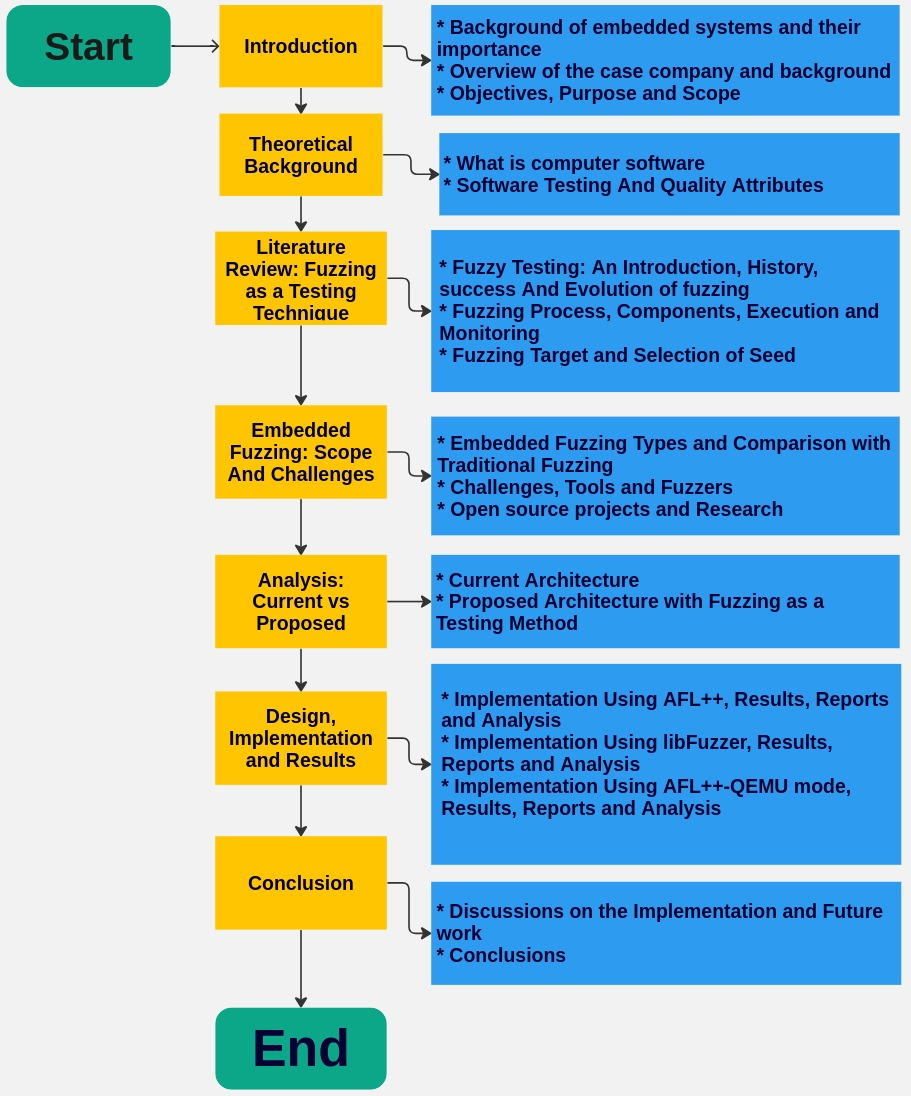
\includegraphics{illustration/thes_str.png}}}
      \caption{Thesis Flow Chart}\label{fig:thes_str}
\end{figure}

\clearpage